%%%%%%%%%%%%%%%%%%%%%%%%%%%%%%%%%%%%%%%%%
% Thin Sectioned Essay
% LaTeX Template
% Version 1.0 (3/8/13)
%
% This template has been downloaded from:
% http://www.LaTeXTemplates.com
%
% Original Author:
% Nicolas Diaz (nsdiaz@uc.cl) with extensive modifications by:
% Vel (vel@latextemplates.com)
%
% License:
% CC BY-NC-SA 3.0 (http://creativecommons.org/licenses/by-nc-sa/3.0/)
%
%%%%%%%%%%%%%%%%%%%%%%%%%%%%%%%%%%%%%%%%%

%----------------------------------------------------------------------------------------
%	PACKAGES AND OTHER DOCUMENT CONFIGURATIONS
%----------------------------------------------------------------------------------------

\documentclass[a4paper, 11pt]{article} % Font size (can be 10pt, 11pt or 12pt) and paper size (remove a4paper for US letter paper)
\usepackage[ngerman]{babel}
\usepackage[protrusion=true,expansion=true]{microtype} % Better typography
\usepackage{graphicx} % Required for including pictures
\usepackage{wrapfig} % Allows in-line images

\usepackage{mathpazo} % Use the Palatino font
\usepackage[T1]{fontenc} % Required for accented characters
\linespread{1.05} % Change line spacing here, Palatino benefits from a slight increase by default

\usepackage[utf8]{inputenc}
\usepackage[colorlinks, pdfpagelabels, pdfstartview = FitH, bookmarksopen = true, bookmarksnumbered = true, linkcolor = black, plainpages = false, hypertexnames = false, citecolor = black] {hyperref}
\usepackage{hyphenat}

\makeatletter
\renewcommand\@biblabel[1]{\textbf{#1.}} % Change the square brackets for each bibliography item from '[1]' to '1.'
\renewcommand{\@listI}{\itemsep=0pt} % Reduce the space between items in the itemize and enumerate environments and the bibliography

\renewcommand{\maketitle}{ % Customize the title - do not edit title and author name here, see the TITLE block below
\begin{flushright} % Right align
{\LARGE\@title} % Increase the font size of the title

\vspace{50pt} % Some vertical space between the title and author name

{\large\@author} % Author name
\\\@date % Date

\vspace{40pt} % Some vertical space between the author block and abstract
\end{flushright}
}

\usepackage{tabularx}

%-----------------------
% Header
%--------------------
\usepackage{fancyhdr}
\pagestyle{fancy}
\fancyhf{}
\fancyhead[L]{
	
\includegraphics[scale=0.1]{./images/logo.png}
}

%----------------------------------------------------------------------------------------
%	TITLE
%----------------------------------------------------------------------------------------

\title{\textbf{Dokumentation des Medida Projekts "Uniknigge"}\\ % Title
von Hung Tran Duc, Elizaveta Ragozina, Philipp Plotz, Christoph Jurkowski, Niklas Fallik und Sheyda Hayatgheybi} % Subtitle

\author{\textsc{Gruppe 1 (Tutorin: Bianca Preißler)} % Author
\\{\textit{Technische Universität Dresden}}} % Institution

\date{18.07.2015} % Date

%----------------------------------------------------------------------------------------

\begin{document}

\maketitle % Print the title section

%----------------------------------------------------------------------------------------
%	ABSTRACT AND KEYWORDS
%----------------------------------------------------------------------------------------

\renewcommand{\abstractname}{Präambel} % Uncomment to change the name of the abstract to something else

\vspace{5cm} % Some vertical space between the abstract and first section


\begin{abstract}
\noindent
Die hier vorliegende Dokumentation des Mediendidaktik und -psychologie Praktikums der Gruppe 1 mit Hung Tran Duc, Elizaveta Ragozina, Philipp Plotz, Christoph Jurkowski, Niklas Fallik und Sheyda Hayatgheybi legt die Vorstellung des Spiels, die technische Umsetzung, die Evaluation mit der Zielgruppe, den Projektverlauf
und das eigene Fazit sowie ein Statement von jedem Gruppenmitglied dar. Das Lernspiel "Uniknigge" basiert auf dem weitverbreiteten Adobe Flash und bildet zusammen mit diversen Mini-Spielen und Grafiken ein vollständiges Spiel.
\end{abstract}

% \hspace*{3,6mm}\textit{Keywords:} lorem , ipsum , dolor , sit amet , lectus % Keywords

%----------------------------------------------------------------------------------------
%	ESSAY BODY
%----------------------------------------------------------------------------------------

\newpage
\renewcommand{\contentsname}{Inhaltsverzeichnis}
\tableofcontents

\newpage
\section{Einführung}
Diese Dokumentation besschreibt die Umsetzung des Lernspiels "Uniknigge" von der Idee bis zum vollständigen Spiel durch die Entwickler und Grafiker Hung Tran Duc, Elizaveta Ragozina, Philipp Plotz, Christoph Jurkowski, Niklas Fallik und Sheyda Hayatgheybi.

\section{Vorstellung des Spiels}
\subsection{Allgemein}
Unsere Grundidee war es ein Lernspiel zu entwickeln, welches als universalen Verhaltenskodex für angehende Studenten am Beispiel eines Informatikstudenten der TU Dresden dient. Angelehnt an den Verhaltenskodex haben wir unser Spiel „Uniknigge“ genannt. Unsere Zielgruppe sind angehende Studenten, die kurz vor dem Antritt ihres Erststudiums sind, d.h. zwischen der Immatrikulation und dem ersten Tag in der Universität. Dabei benötigt der Spieler keinerlei spezifische Vorkenntnisse, sondern soll intuitiv nach bestem Gewissen agieren. \\

Das Spiel selbst führt den Spieler durch einen fiktiven ersten Tag in der Uni und stellt ihn immer wieder vor soziale wie auch intellektuelle Herausforderungen. Die Herausforderungen werden in der Spielstory wie auch in den Minispielen offensichtlich oder versteckt gestellt. Während des Intros wird dem Spieler in Form einer Smartphone App eine ausführliche Erklärung, welche man jederzeit im Spiel wieder aufrufen kann, zur Verfügung gestellt. Zusätzlich werden vor jedem Minispiel, weitere Regeln zum Verhalten wie auch zur Spielanwendung bereitgestellt. Nach den Minispielen sowie bei Herausforderungen während des Spiels, wird eine kurze Auswertung gezeigt, ggf. mit Lob und Kritik. Am Ende des Spiels folgt eine längere Resolution mit Verweisen auf jeweilige Herausforderungen mit Verbesserungsvorschlägen für den nächsten Spielablauf. Da unser Spiel eine Verhaltensanleitung darstellt, ist das Ziel und die Zielfindung zunächst nicht klar erkennbar und wird erst während des Spiels sichtbar.
Das Ziel ist es, eine Balance zwischen dem aufmerksamen, leistungsfokussierten Lernen und den für das Studium überlebenswichtigen Sozialkompetenzen zu erreichen.

\subsection{Spiel}
\subsubsection{Startmenü}
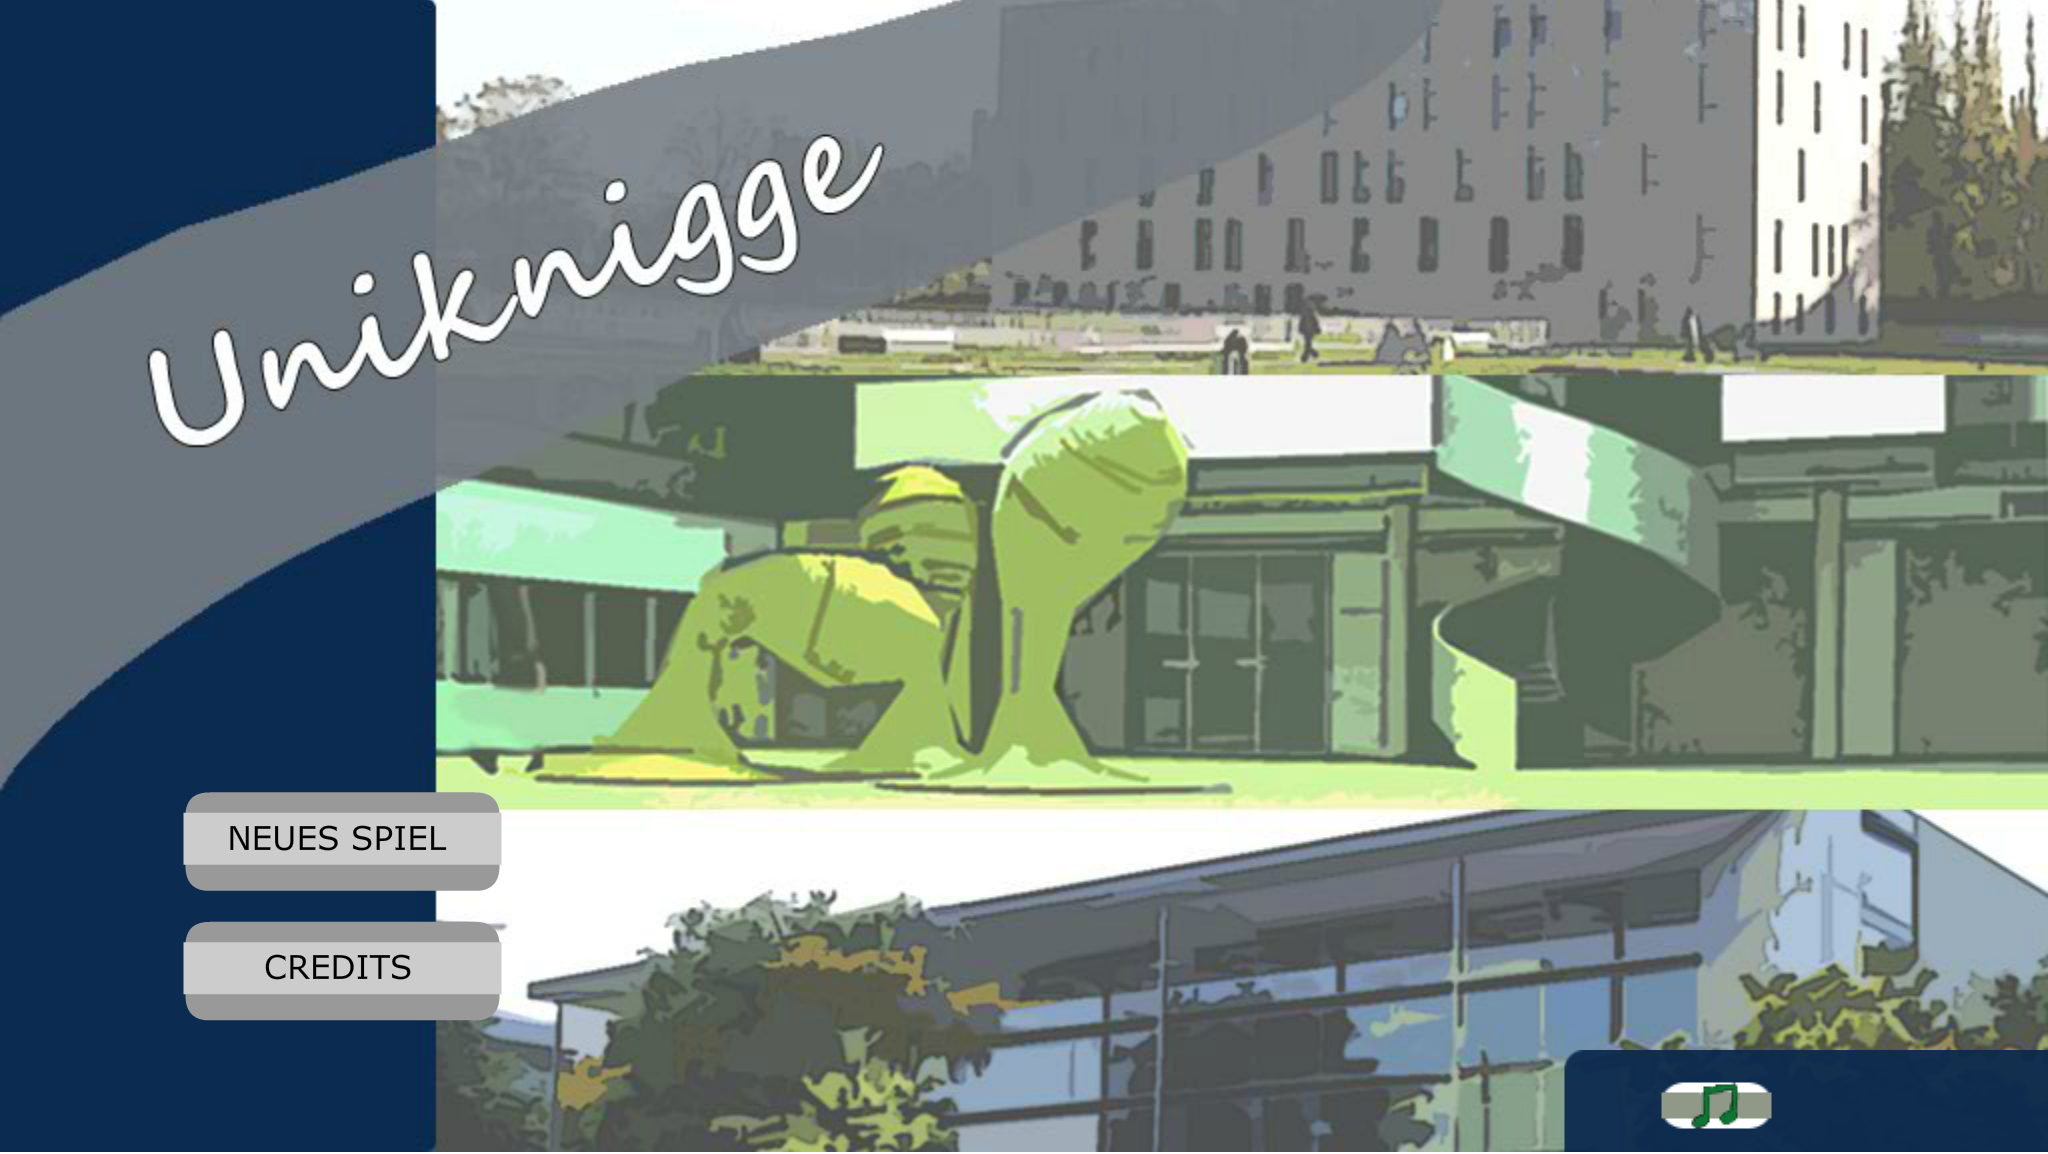
\includegraphics[scale=0.46]{images/spiel/startmenue.png}\\\\
Wenn das Spiel gestartet wird, kann hier der ins Spiel einsteigen. Am Rand unten links findet der Spieler Buttons um den Ton zu steuern oder das Spiele zu pausieren.

\subsubsection{Einleitung}
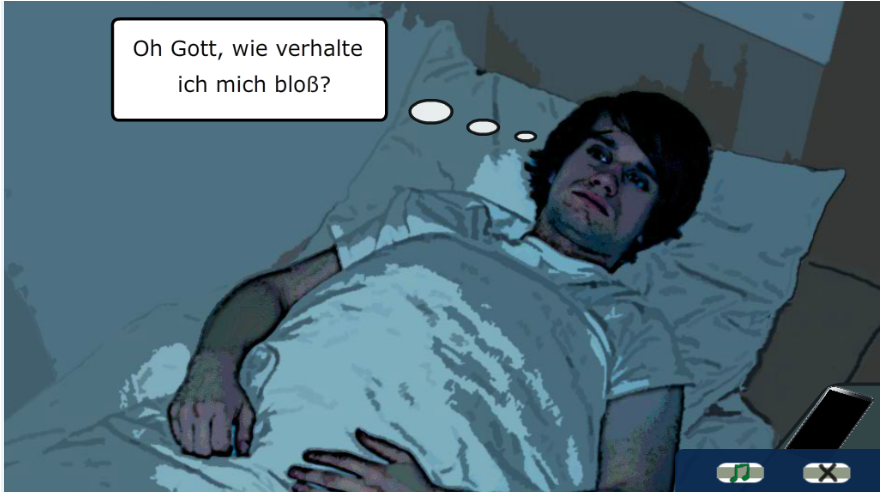
\includegraphics[scale=0.535]{images/spiel/2.png}\\\\
Am Anfang des Spiels wird der Spieler in das Spielgeschehen eingeführt. In einer kurzen Animierten Einleitung kann der Spieler seine aktuelle Position im Spiel erfahren. Nebenbei werden ihm die Element zur Bedienung des Spiels vorgestellt.

\subsubsection{Busspiel}
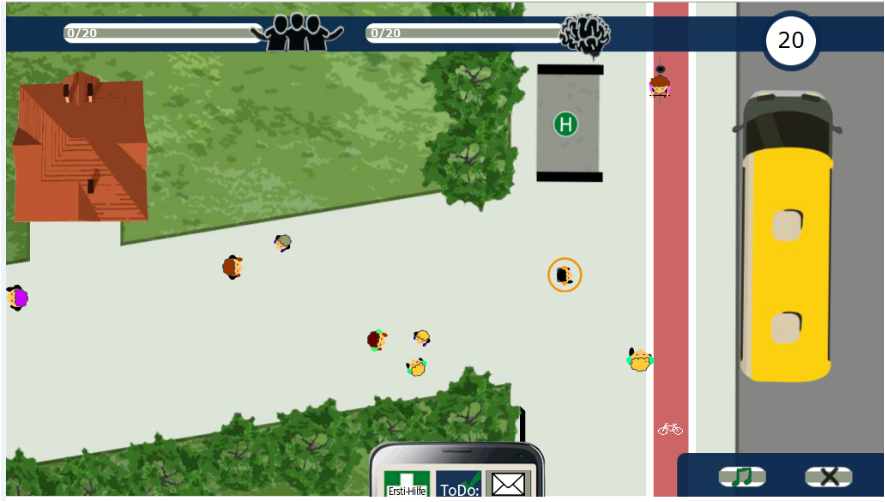
\includegraphics[scale=0.535]{images/spiel/3.png}\\\\
Aufgabe in diesem Spiel ist es in der vorgegebenen Zeit den Bus zu erreichen, ohne dabei einen Passanten zu anzurempeln. Die Steuerung funktioniert mit den Pfeiltasten. Wie in fast jedem von unseren Minispielen, soll dem Spieler die Balance zwischen Sozialem und dem striktem Unistoff beigebracht werden. Hier ist wichtig, dass sich der Spieler nicht nur auf den Bus konzentriert, der ihn schnell und rechtzeitig zur Vorlesung bringt, sondern auch auch auf seine Mitmenschen. Er bekommt nur wenig bis keine Sozialpunkte, wenn er den Bus erreicht und dabei viele Menschen anrempelt. Ebenso wie der Spieler weniger Wissenspunkte erhält, wenn der ein Bus nicht erreicht.

\subsubsection{Vorlesung 1 und 2}
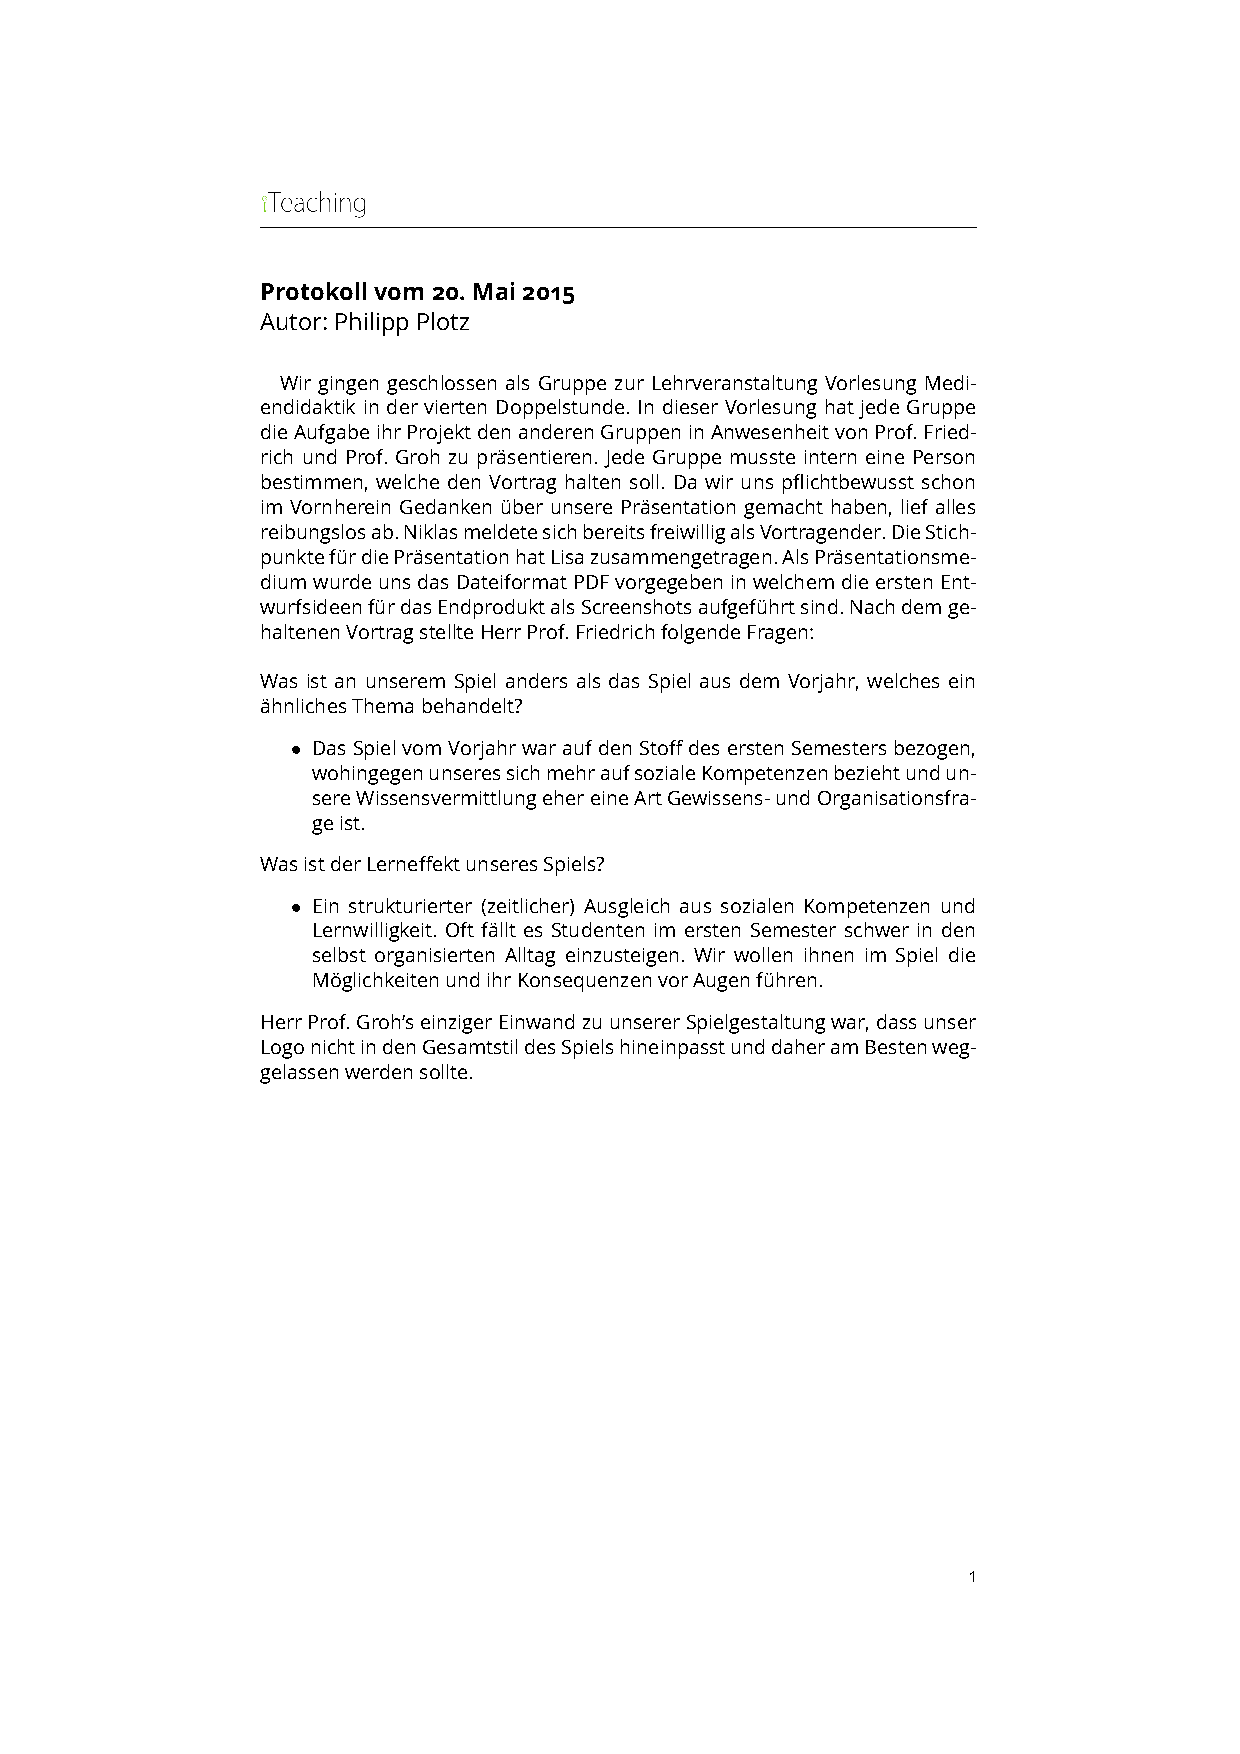
\includegraphics[scale=0.535]{images/spiel/5.png}\\\\
Dieses Spiel ist in zwei Vorlesungen geteilt, in der Ersten soll den Spieler Aufmerksamkeit und Wissen, vermittelt und beigebracht werden. Dieses Wissen wird zu einen späteren Zeitpunkt (Übung) abgefragt. Der erste Teil ist eine „Point-and-Klick“ Prinzip. \\
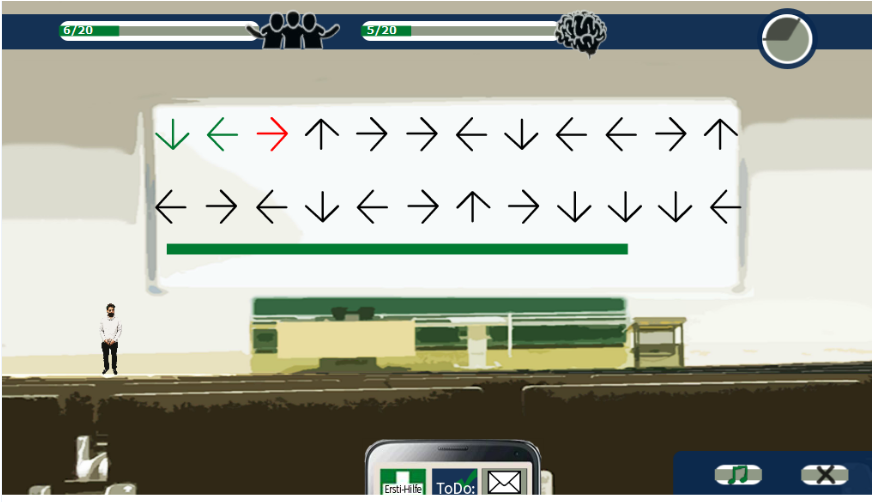
\includegraphics[scale=0.535]{images/spiel/15.png}\\\\
In der zweiten Hälfte soll dem Spieler der zweite elementare Baustein zur Wissensaufnahme vermittelt werden, das Mitschreiben von Notizen. Umgesetzt haben wir die Idee des Mitschreibens durch Drücken der entsprechenden, auf der Tafel angezeigten Pfeiltasten. Es ist zwar möglich durch Konversationen und abbrechen der Vorlesung Sozialpunkte zu sammeln, doch haben wir hier eigentlich das Augenmerk auf die Wissensvermittlung und dadurch auch auf die Wissenspunkte gesetzt.

\subsubsection{Mensa}
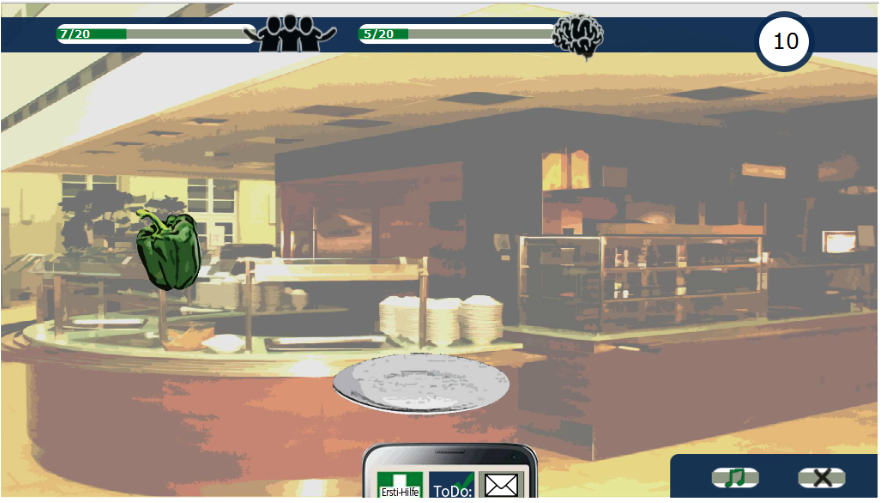
\includegraphics[scale=0.535]{images/spiel/8.png}\\\\
Im Gegensatz zum Vorlesungsspiel, haben wir uns hier mehr auf die Sozialpunkte fokussiert. Ein Mädchen stolpert in der Mensa und der Spieler muss ihr helfen, das noch fliegende Essen, wieder einzusammeln. Um das Essen aufzufangen, steuert man einen Teller mit den Pfeiltasten. Bewusst haben wir hier eine dritte Person gewählt die stolpert und nicht unseren Protagonisten, um dem Spieler zu zeigen, dass er sich seinem sozialen Umfeld öffnen sollte. 
\subsubsection{Labyrinth}
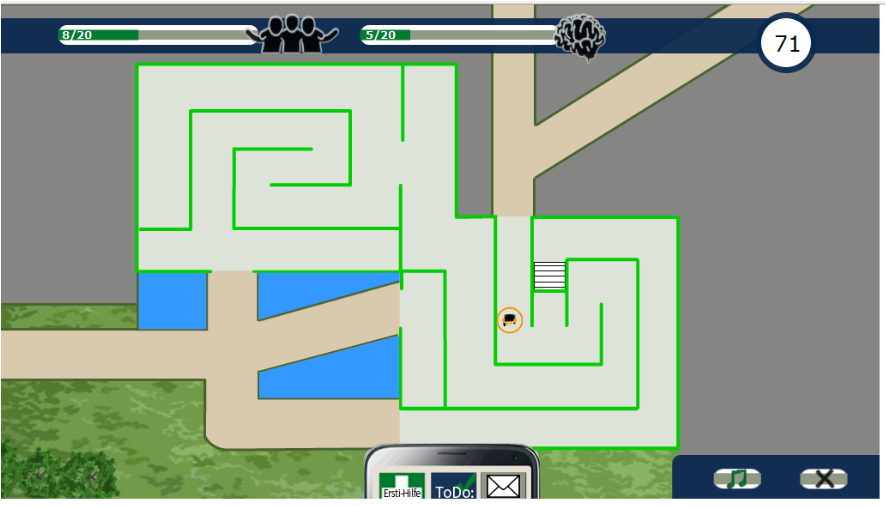
\includegraphics[scale=0.535]{images/spiel/9.png}\\\\
Dieses Spiel spiegelt, eine für jeden Studenten bekannte Situation wieder, deshalb hielten wir diese Anwendung für unentbehrlich. Wieder ist von dem Spieler gefordert, in einer bestimmten Zeit etwas zu erreichen, hierbei handelt es sich um einen Übungsraum. Die Suche führt durch die Informatik Fakultät leicht abgewandelt als Irrgarten. Gesteuert wir die Spielfigur mit den Pfeiltasten.

\subsubsection{Übung}
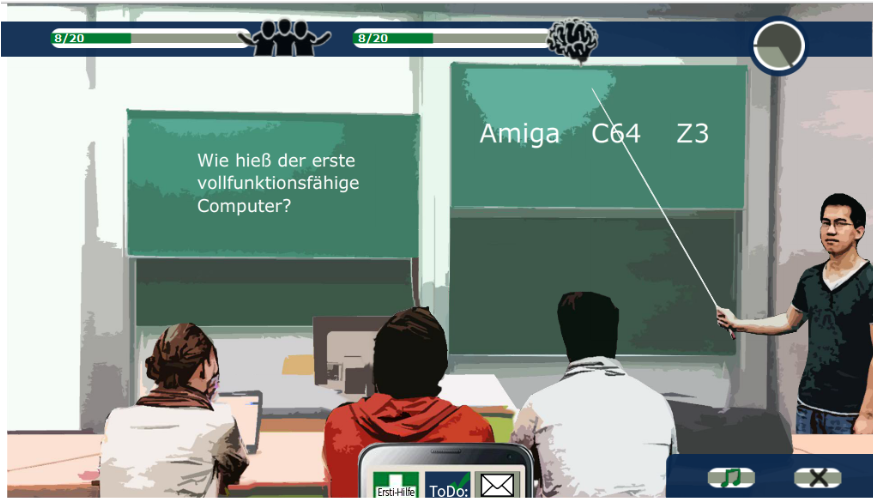
\includegraphics[scale=0.535]{images/spiel/11.png}\\\\
Die Übung ist als Wiederholung der Vorlesung gedacht. Durch einfache Fragen im Bezug auf die Vorlesung kann der Spieler hier sein gelerntes wissen überprüfen. Der Spieler erhält durch Animation des Tutor direkt ein Feedback auf seine Antworten. Auf Richtig beantwortete Fragen erhält der Spieler als Belohnung Punkte.

\subsubsection{Entscheidung}
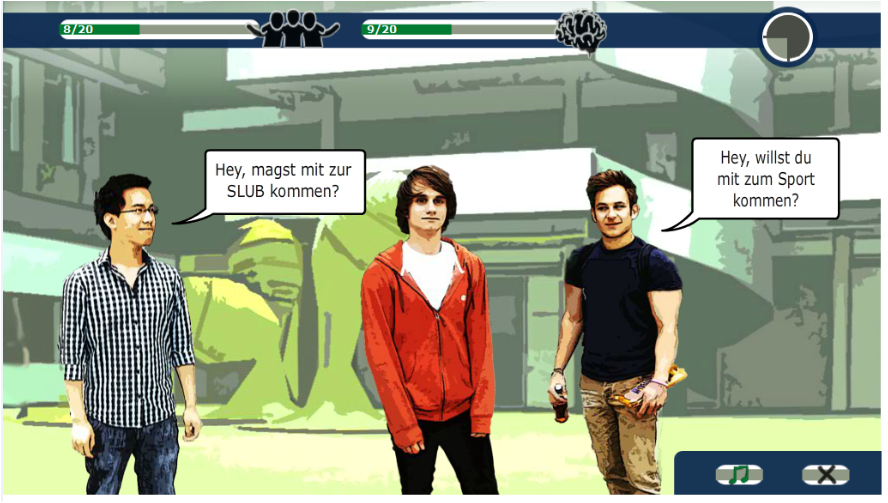
\includegraphics[scale=0.535]{images/spiel/12.png}\\\\
Nach der Übung kann der Spieler etwas über die Möglichkeiten zur Freizeitgestaltung lernen. Je nach Auswahl erhält der Spieler eine andere Belohnung.

\subsubsection{Abschluss}
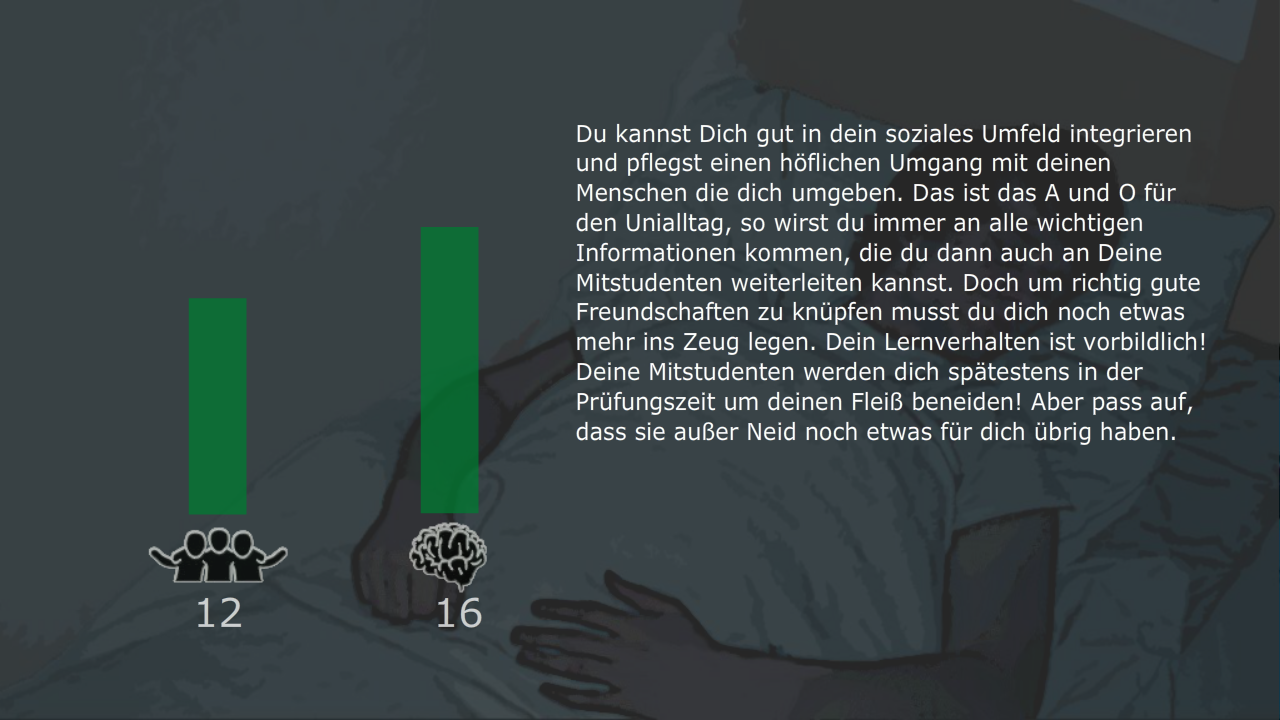
\includegraphics[scale=0.46]{images/spiel/outro.png}\\\\
Am Ende des Spiels werden dem Spieler seine Punkte nach einer kleinen Animation angezeigt. Zu seinen Punkten erhält der Spieler auch einen kurzen Erklärungstext.

\section{Technische Umsetzung}
\subsection{Layout}
Das Spiel ist im Comicdesign gehalten um den Spieler in einer spielerischen und nicht ganz realistischen Welt der Hochschulen und Universitäten zu empfangen. Durch die Wahl des Comicdesign wird auch die Gestaltung des Spieles Vereinfacht und die Entwicklung beschleunigt. Durch statische Schaltflächen die zu jeder Zeit im Spiel vorhanden sind kann zum Beispiel die Audioausgabe gesteuert, oder das Spiel pausiert werden. Durch Sprech- und Gedankenblasen kann der Spieler dem Spielablauf gut folgen. Damit der Spieler auch im Verlauf des Spiels nachlesen kann, was er zu tun hat, wurde zusätzlich in Smartphone mit hilfreichen Informationen eingebaut. Damit der Spieler das Spiel intuitiv bedienen kann wurde zusätzlich auf die Konsistenz der Benutzersteuerung wert gelegt.

\subsection{Hauptmenü}
Unser Hauptmenü, wie auch alle weiteren Spielsequenzen haben als Hintergrund ein Foto, das in Photoshop bearbeitet, an eine Comic-ähnliche Aufmachung erinnert. Diesen Stil haben wir auch auf die Figuren und sämtliche andere Gegenstände übertragen.
Zusätzlich ist im Hauptmenü der Schriftzug „Uniknigge“ und drei Buttons zu sehen. Die Buttons sind zum Starten des Spiels, Fortsetzen des Spiels und zur aktuellen Punkteabfrage vorgesehen. Das Hauptmenü dient der Einstimmung des Spielers auf das Spiel und die Spielumgebung.

\subsection{Einleitung}
Wie bereits erwähnt, zieht sich unser Layout aus Comic-ähnlichem Bildmaterial durch das ganze Spiel. Das Intro ist eine kleine Filmsequenz, der den Spieler in die Problematik und Aufgabenstellung, wie auch Anwendungen beispielsweise das Smartphone, einführt. Zu sehen ist ein Student, der vor seinem ersten Unitag nicht schlafen kann. Um ihm die Angst zu nehmen, bekommt er eine Kurznachricht. Auf seinem Smartphone kann er so Regeln, Anweisungen und Tipps einsehen.

\subsection{Spielablauf}
Der Spielablauf ist als "Point-and-Click“ Anwendung konzipiert. Entscheidungsfragen, häufig eingeleitet durch einen virtuellen Kommilitonen, werden in Form von Sprechblasen dargestellt.
Auch die Punkteübersicht und der zeitliche Fortschritt des gesamten Spiels sind zu jeder Zeit in Form von Balken bzw. einer Uhr sichtbar.

\subsection{Minispiele}
Bezüglich des Designs sind die Minispiele im gewohnten Comic-Layout gehalten, doch im Gegensatz zu dem herkömmlichen Spielablauf werden hierfür die Pfeiltasten zur Bedienung bemüht. Das hat den Effekt, dass der Spieler merkt, dass ihm bei diesen Aufgaben mehr abverlangt wird, als im sonstigen Spielablauf. Zudem kann er die Maus benutzen, um die Anwendung zu pausieren.

\subsection{Smartphone}
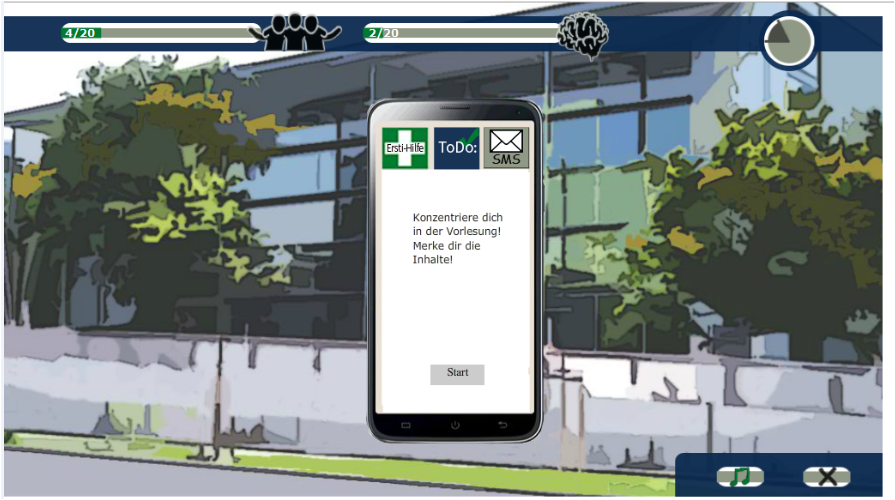
\includegraphics[scale=0.535]{images/spiel/4.png}\\\\
Das Smartphone dient als Informationsquelle. Zu jedem Zeitpunkt während des Spiels bietet es dem Spieler die Möglichkeit Fakten und Verhaltensregeln im Allgemeinen oder auch zur spezifischen Situation nachzulesen.

\subsection{Abschluss}
Der Abschluss ist an das Intro angelehnt. Der Student befindet sich nach seinem ersten Tag wieder in seinem Bett, wo er seinen ersten Tag an der Uni Revue passieren lässt. Er bekommt über seine Smartphone-App die Evaluation mit Tipps und Anmerkungen zu seinen Entscheidungen. 

\subsection{Hilfsmittel für die Entwicklung}
\begin{tabular}{lp{9cm}}
\textbf{Programm} & \textbf{Bemerkungen} \\ 

\includegraphics[scale=0.35]{images/flash.png} & 
\nohyphens{
Adobe Flash CC 2014 für die Umsetzung des Spiels
(Funktionalitäten, Animationen, Navigation)
} \\

\includegraphics[scale=0.5]{images/photoshop.png} & 
\nohyphens{
Adobe Photoshop CC 2014 für die Bildbearbeitung und die Erstellung von Grafiken
} \\

\includegraphics[scale=0.13]{images/flash_player.png} & 
\nohyphens{
Adobe Flash Player zur Ausführung des Spiels
} \\
\end{tabular} 

\subsection{Hilfsmittel für die Kommunikation}
\begin{tabular}{lp{9cm}}
\textbf{Programm} & \textbf{Bemerkungen} \\ 

\includegraphics[scale=0.22]{images/git.png} & 
\nohyphens{
Git als Versionsverwaltungswerkzeug
} \\\\

\includegraphics[scale=0.099]{images/facebook.png} & 
\nohyphens{
Facebook zur Absprache und Organisation beispielsweise von Treffen und Erklärung spontaner Fragen
} \\
\end{tabular} 

\subsection{Quellen der verwendeten Medien}

\begin{tabular}{|lllllp{4.5cm}|}
\hline 
\textbf{Wo?} & \textbf{Format} & \textbf{Object} & \textbf{Autor(en)} & \textbf{Lizenz} & \textbf{Quelle} \\ 
\hline
S & B & H & iTeaching & CC & - \\ 
\hline
S & SD & H & Pitx & CCBY3.0 & [CCM]/Pitx/15328 \\ 
\hline
MS & SD & H & unreal\b{ }dm & CCBY2.5 & [CCM]/unreal\b{ }dm/33850 \\ 
\hline
V1 & B & HSZ & Hans-Jürgen Räth & PublicDomain & de.ikipedia.org \\
\hline
V1 & B & H & iTeaching & CC & - \\ 
\hline
V1 & B & Student & iTeaching & CC & - \\ 
\hline
V2 & B & H & iTeaching & CC & - \\ 
\hline
V2 & B & Student & iTeaching & CC & - \\ 
\hline
M & B & Essen & Pixabay.com & CC0 & Pixabay.com \\ 
\hline
M & SD & Essen & iTeaching & CC & - \\ 
\hline
M & B & H & iTeaching & CC & - \\ 
\hline
M & B & Student & iTeaching & CC & - \\ 
\hline
L& SD & H & iTeaching & CC & - \\ 
\hline
L& B & Student & iTeaching & CC & - \\ 
\hline
Ü& B & H & iTeaching & CC & - \\ 
\hline
Ü& B & Student & iTeaching & CC & - \\ 
\hline
\end{tabular} \\\\
Legende \\
\begin{tabular}{|lp{6cm}|}
\hline 
\textbf{Abkürzung} & \textbf{Volltext} \\
\hline 
S & Startmenü \\
MS & Minispiele \\
V1 & Vorlesung 1 \\
V2 & Vorlesung 2 \\
M & Mensa \\
L & Labyrinth \\
Ü & Übung \\
B & Bild \\
SD & Sound \\
CCM & http://dig.ccmixter.org/files/* \\
H & Hintergrund \\
\hline
\end{tabular}


\section{Evaluation mit der Zielgruppe}
\subsection{Allgemeines}
Das Lernspiel gibt angehenden Studenten, die zwischen der Immatrikulierung und der ersten Vorlesungszeit stehen die Möglichkeit den Unialltag spielerisch in seiner Vielseitigkeit kennenzulernen. Ausgerichtet auf diesen Anspruch haben wir die Bedienungen, Texte und Aufgaben auf einem hohen Niveau, damit sie die angehenden Studenten damit identifizieren können. Neben dem spielerischen Aspekt kann das Lernspiel auch auf den Webseiten von Universitäten und Berufsorientierungsportalen zu Verfügung gestellt werden. Abiturienten können durch das Spiel Fragen wie zum Beispiel "Wie sieht der Unialltag aus?“, "Wie finde ich mich an der Uni zurecht?“ oder "Wie komme ich in Kontakt mit anderen Studenten?“ klären. Um Spielatmosphäre während des Spielens und Lernen etwas aufzulockern, Haben fiktive Elemente, wie Karlchen, welcher dem Spieler Nachts die Smartphone App empfiehlt, eingebaut. Zudem sind die Minispiele überzogene Anlehnungen an unsere eigenen Erfahrungen an das erste Semester. Ein Beispiel das jeder Student kennt ist das Labyrinth zur Raumfindung. 

\subsection{Fragebogen}
Zur Evaluierung unseres Projekts haben wir einen Fragebogen erstellt und an Bekannte verteilt die gerade mit Abitur fertig geworden sind und mit dem Gedanken Spielen ein Studium aufzunehmen. \\\\
Dies ist das Ergebnis: \\
\begin{tabular}{|lp{0.19cm}|}
\hline 
\textbf{Frage} & \textbf{\O} \\
\hline 
Fandest Du das Spiel hilfreich um einen Einblick in den & \\
Unialltag zu gewinnen? & 4 \\
Fandest Du das Spiel hat Dir die Balancelehre des Studiums & \\
vermitteln können? & 5 \\
Ist es Dir schwer gefallen bei dem Spiel eine hohe Punktzahl & \\
zu erlangen? & 2 \\
Würdest Du Dir wünschen, dass das Spiel an Berufsberatungsstellen & \\
zur Verfügung steht? & 4 \\
Fandest Du, dass die Texte und Anforderungen für deiner & \\
 Altersgruppe entsprachen? & 3 \\
\hline
\end{tabular} \\\\
Legende \\
\begin{tabular}{|lp{3cm}|}
\hline 
\textbf{Abkürzung} & \textbf{Volltext} \\
\hline 
1 & Leider gar nicht \\
2 & Überwiegend nicht \\
3 & Teils teils \\
4 & Meistens \\
5 & Ja, auf jeden Fall \\
\hline
\end{tabular}

\section{Projektverlauf}
\subsection{Aufgabenverteilung}
\begin{tabular}{|lp{9.0cm}|}
\hline 
\textbf{Mitglied} & \textbf{Aufgaben} \\ 
\hline 
Hung Tran Duc & Smartphone, Hauptspiel, Vorlesung 2, Gruppenleiter  \\ 
\hline
Elizaveta Ragozina & Einleitung, Busspiel, Hauptspiel, Design \\ 
\hline
Philipp Plotz & Vorlesung 1, Abschluss, Protokollant \\ 
\hline
Christoph Jurkowski & Übung, Entscheidung, Smartphone, Dokumentation \\ 
\hline
Niklas Fallik & Labyrinth, Hauptspiel, Mensaspiel \\ 
\hline
Sheyda Hayatgheybi & Mensaspiel, Dokumentation \\ 
\hline

\end{tabular} 

\subsection{Zeitplan}
Zeitplanung am Anfang des Praktikums:
\begin{figure}[ht]
	\makebox[\textwidth]{ 
	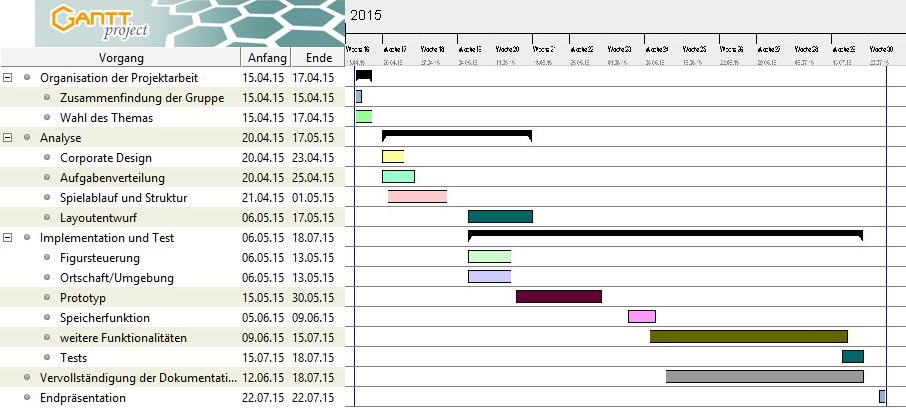
\includegraphics[scale=0.65]{./images/proj2.jpg}}
\end{figure} \\\\
Die Zeitplanung hat sich im laufe des Semesters verschoben. Dafür gab es im Semester verschiedene Gründe wie Praktika für das Fach Medienströme oder das Komplexpraktikum und andere Vorlesungen. Zum Teil wurden auch einzelne Minispiele in ihrem Arbeitsaufwand unter und überschätzt. Zum Ende des Praktikums konnte schließlich alle Teile fertig gestellt werden. Aufgrund des immensen zeitaufwandes für die Vorbereitung und Aufzeichnung von Stimmen für die einzelnen Spielfiguren wurde davon Abstand genommen.

\subsection{Aufwandsabschätzung}

\vspace{5pt}
\begin{tabularx}{\textwidth}{ccXrr}
\hline
%\rowcolor[gray]{.95}
\tiny {Menge} & \tiny {Einheit} & \tiny {Beschreibung} & \tiny {Einzelpreis (netto)} & \tiny {Gesamtpreis (netto)} \\ \hline
 400 & Std. & Arbeit & \multicolumn{1}{r}{62,00 EUR} & \multicolumn{1}{r}{24800,00 EUR} \\ \hline \hline
\multicolumn{ 4}{l}{\small{Summe ohne MwSt.}} & 24800,00 EUR \\ \hline
\multicolumn{ 4}{l}{\small{MwSt. 19\% }} & 4712,00 EUR \\ \hline \hline
\multicolumn{ 4}{l}{ \textbf{Gesamtsumme inkl. MwSt.} } & \textbf{29512,00 EUR} \\ \hline
\end{tabularx}


\subsection{Kostenabschätzung}

\vspace{5pt}
\begin{tabularx}{\textwidth}{ccXrr}
\hline
%\rowcolor[gray]{.95}
\tiny {Menge} & \tiny {Einheit} & \tiny {Beschreibung} & \tiny {Einzelpreis (netto)} & \tiny {Gesamtpreis (netto)} \\ \hline
\multicolumn{ 4}{l}{\small{Software}} & 856,56 EUR \\ \hline
 6 & St. & Adobe Creative Cloud April & \multicolumn{1}{r}{35,69 EUR} & \multicolumn{1}{r}{214.14 EUR} \\ \hline \hline
 6 & St. & Adobe Creative Cloud Mai & \multicolumn{1}{r}{35,69 EUR} & \multicolumn{1}{r}{214.14 EUR} \\ \hline \hline
 6 & St. & Adobe Creative Cloud Juni & \multicolumn{1}{r}{35,69 EUR} & \multicolumn{1}{r}{214.14 EUR} \\ \hline \hline
 6 & St. & Adobe Creative Cloud Juli & \multicolumn{1}{r}{35,69 EUR} & \multicolumn{1}{r}{214.14 EUR} \\ \hline \hline
\multicolumn{ 4}{l}{\small{Projektkonzeption}} & 6200,00 EUR \\ \hline
 1 & St. & Themenentwurf & \multicolumn{1}{r}{700.00 EUR} & \multicolumn{1}{r}{700.00 EUR} \\ \hline \hline
 1 & St. & Grafikentwurf & \multicolumn{1}{r}{2500.00 EUR} & \multicolumn{1}{r}{2500.00 EUR} \\ \hline \hline
 1 & St. & Spielentwurf & \multicolumn{1}{r}{3000.00 EUR} & \multicolumn{1}{r}{3000.00 EUR} \\ \hline \hline
\multicolumn{ 4}{l}{\small{Projektumsetzung}} & 10500,00 EUR \\ \hline
 1 & St. & Bearbeitung der Grafiken & \multicolumn{1}{r}{1500.00 EUR} & \multicolumn{1}{r}{1500.00 EUR} \\ \hline \hline
 1 & St. & Lerntexte & \multicolumn{1}{r}{2000.00 EUR} & \multicolumn{1}{r}{2000.00 EUR} \\ \hline \hline
 1 & St. & Funktionalitäten & \multicolumn{1}{r}{7000.00 EUR} & \multicolumn{1}{r}{7000.00 EUR} \\ \hline \hline
\multicolumn{ 4}{l}{\small{Projektoptimierung}} & 1000,00 EUR \\ \hline
 1 & St. & Optimierung & \multicolumn{1}{r}{500.00 EUR} & \multicolumn{1}{r}{500.00 EUR} \\ \hline \hline
 1 & St. & Dokumentation & \multicolumn{1}{r}{500.00 EUR} & \multicolumn{1}{r}{500.00 EUR} \\ \hline \hline
\multicolumn{ 4}{l}{\small{Summe ohne MwSt.}} & 18556,56 EUR \\ \hline
\multicolumn{ 4}{l}{\small{MwSt. 19\% }} & 3525,75 EUR \\ \hline \hline
\multicolumn{ 4}{l}{ \textbf{Gesamtsumme inkl. MwSt.} } & \textbf{22082,31 EUR} \\ \hline
\end{tabularx}

\section{Fazit}
Am Ende unseres Prakrikums haben wir viel über das Entwickeln von Spielen in Flash gelernt. Leider haben nun erste Browserhersteller, wie Firefox, Flash standardmäßig auf Grund von Sicherheitslücken deaktiviert. Dennoch können wir mit den gewonnen Erfahrungen in zukünftigen Projekten Aufgabenstellungen noch besser einschätzen. Da die Zeit nur sehr kurz war konnten wir leider nicht alle Idee umsetzen. Es wäre Vorstellbar unser Spiel auf andere Universitäten und Studiengänge anzupassen. Es könnten auch noch Text eingesprochen werden und weiter Minispiele entwickelt werden. Am liebsten hätten wir noch unserer Spiel weiter perfektioniert.

\section{Statement von jedem Gruppenmitglied}
\subsection{Hung Tran Duc}
Das Praktikum hatte eine interessante Aufgabenstellung und lies Raum für kreative Spielideen.
Allerdings ist der zeitliche Aufwand sehr hoch für die angegebene 1 SWS.
Wie erwartet konnte man den Zeitplan nicht einhalten, es fehlte einem zu Beginn des Praktikums schlichtweg 
die Erfahrung um so etwas planen und vorhersagem zu können.
In der Gruppe selbst gab es Probleme bei der Arbeits- und Aufgabenverteilung.
Unsere Tutorin war hilfreich und leicht erreichbar.

\subsection{Elizaveta Ragozina}
Durch das Praktikum konnte man eigene Erfahrung im Bereich Spielentwicklung mit Adobe Flash machen. Da ich mit anderen Adobe Produkten schon vertraut war und am Lernen der Flash-Funktionsweisen interessiert war, war meine Einarbeitungszeit vergleichsweise gering. Das Designen hat auch sehr viel Spaß gemacht und ich konnte viele neue Erfahrungen mit den verwendeten Programmen sammeln. Zwar konnte ich in der Gruppe das Konsistenzkonzept, aufgrund von unterschiedlichen Vorstellungen und Zeitmangel für unser Spiel nicht vollständig durchsetzen, dennoch gefällt mir das Endprodukt sehr.
Noch zu erwähnen ist, dass unsere Gruppenarbeit bei weiten nicht perfekt war, was teilweise an längerer Einarbeitungszeit, teilweise an fehlender Motivation einiger Gruppenmitglieder lag. Das führte dazu, dass ein Teil der Gruppe einen großen Anteil der Aufgaben Anderer übernehmen mussten und so sehr viel mehr zum Endergebnis beigetragen haben. Mein Zeitaufwand lag ungefähr beim Vier- bis Fünffachem vom Vorgesehenem und war damit dem Zeitaufwand beim SWT-Praktikum aus dem 2. Semester ähnlich. Ich denke auch, wenn alle Gruppenmitglieder gleich viel beitragen würden, wäre der Zeitaufwand für dieses Spiel höher als der Vorgesehene. Aus meiner Sicht ist es umso mehr Schade, das der Einfluss auf die Modulnote in keinem Vergleich zur aufgewendeten Zeit steht. \\
Alles in allem war das Projekt sehr lehrreich. Die Spielentwicklung hat mich begeistert. Ich kann mir vorstellen, mein Studium im Bereich der Spielentwicklung zu vertiefen.

\subsection{Philipp Plotz}
Das Praktikum bot mir eine gute Gelegenheit einen Einblick in die Flash Programmierung mit ActionScript3 zu bekommen, welchen ich sonst aus eigenen Stücken nicht vorgenommen hätte. Es war sehr interessant und erstaunlich, wie einfach sich komplexere Mechanismen implementieren ließen und es machte auch nach kurzer Einarbeitungszeit auch Spaß. Leider konnten durch Zeitmangel nicht alle Ideen umgesetzt und der ganze Wille eingebracht werden, was nicht heißen soll, dass das Praktikum zu umfangreich gestaltet ist. Des Weiteren wurden die Arbeitsbedingungen durch intragruppale Konflikte, welche durch unterschiedliche Ansichten vom Endprodukt hervorgerufen wurden, nicht gerade erleichtert. Summa summarum hat sich die Arbeit aus meiner Sicht gelohnt, da ein recht ansehnliches Produkt entstanden ist, welches man gern auch anderen Personen präsentiert. Das Spiel ist konsistent umgesetzt und bietet aus meiner Sicht keine möglichen Kritikpunkte, da allen Anforderungen genüge getan ist.

\subsection{Christoph Jurkowski}
Unter dem Praktikum zur Vorlesung Mediendidaktik und –psychologie konnte ich mir am Anfang nicht viel vorstellen. Nach den ersten Vorlesungen fand ich die Aufgabenstellung sehr interessant. Ich freue mich das unser Projekt durch besonderes Feingefühl in der Gestaltung und Design ein echter Hingucker ist. Durch die schlechte Eigenschaft von Flash, dass man es mit üblichen Versionsverwaltungswerkzeugen nicht managen kann, war des Zusammenführen der einzelnen Projektteile sehr aufwendig. Durch den Einsatz von einzelnen Gruppenmitgliedern konnte das Projekt aber gerettet werden. Das Endergebnis kann sich sehen lassen. \\
Die Strukturierung des Praktikums hätte mehr wie das Softwarearchitektur Praktikum seien sollen. Viele Studenten haben in dieser Phase des Studiums einfach zu wenig Erfahrung in der Entwicklung von Softwareprodukten. Das Praktikum hätte vielleicht durch ein spezielles Tutorium für Flash und HTML5/JavaScript unterstützt werden können. Ein Tutorium zu Projektmanagement oder Konfliktlösungen hätte vielen Gruppen wichtige praktische Soft Skills vermittelt und so die Qualität der Endprodukte gesteigert.


\subsection{Niklas Fallik}
Die Aufgabenstellung habe ich im Hinblick auf den Schwierigkeitsgrad angemessen gefunden.
Die Zwischenpräsentation des Designs war ebenso aufschlussreich wie die ausführlichen Konsultationen unerer Tutorien und die Evaluation mit der Zielgruppe.
In dem Praktikum konnte ich bereits Erlerntes aus den vergangenen Semestern anwenden.
Das zur Umsetzung des Projekts genutzte Adobe Flash mit ActionScript 3.0 bedurfte einer geringen Einarbeitungszeit, sodass ich mit der Impelentierung der mir zugeteilten Aufgaben schnell beginnden konnte.
Zukünftigen Projektgruppen dieses Praktikums würde ich empfehlen, sich einen Team-internen Zeitplan zu erarbeiten und sich streng an diesen zu halten.

\subsection{Sheyda Hayatgheybi}
In meinen Augen bietet das Projekt eine gute Gelegenheit Neues auszuprobieren, da die Vorgaben, wie zum Beispiel die technische Umsetzung und die Spielgeschichte, sehr frei waren. Zudem konnte man direkt das didaktische Wissen mit dem bereits erlernten technischen Kow-how zu verbinden. \\
Trotz, oder vielleicht sogar aufgrund, der sehr freien Angaben zur technischen Umsetzung, war der Arbeitsaufwand während des Semesters enorm hoch, sodass viele unserer Ideen nicht entsprechend umgesetzt werden konnten deshalb finde ich es auch schade, dass das Spiel in der gesamt Note nur sehr gering honoriert wird. 
Die Zusammenarbeit mit unserer Tutorin war für uns eine große Hilfe, da sie uns stets für Fragen, Kritik und Verbesserungsvorschläge zur Verfügung stand.


%----------------------------------------------------------------------------------------

\end{document}